\begin{frame}
	\frametitle{Testes Complementares}
		\framesubtitle{Espalhamento de valores dos vetores de características}

		\begin{columns}
			\column{0.55\textwidth}
			\begin{figure}
				\centering
%				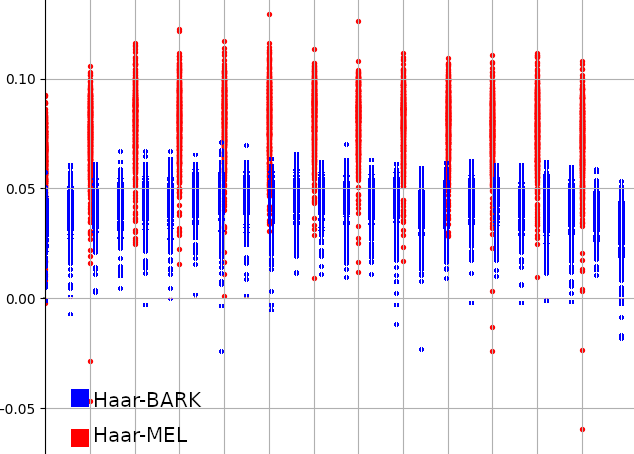
\includegraphics[width=\linewidth]{images/results/BarkVersusMelOnHaar}
				\caption{Espalhamento BARK x MEL para sinais autênticos usando \textit{wavelet} Haar.}
				\label{fig:barkversusmelonhaar}
			\end{figure}
			\column{0.45\textwidth}
			\begin{itemize}
				\item Espalhamento vertical dos valores é maior na escala MEL.
				\item Espalhamento horizontal dos valores é maior na escala BARK.
			\end{itemize}
		\end{columns}		
	
\end{frame}